\chapter{Blockchain}

Predicting the flight delays to set the insurance rates is half the innovation for this new platform. The other half would be overhauling the current insurance's legal aspects. The platform's aim is to make a digital legal agreement between the insurance platform and the user, which is non-repudiable, irrefutable, time-stamped and can be fully trusted by the customers as well as the regulators. Currently the legal agreements involve Notaries and difficult manual legal work, even for a simple agreement. Using Blockchain, creating such a legal agreement could be automated, resulting in efficiency improvements. Before delving into how blockchain forms part of this product, a short introduction to bitcoin and it's core parts will be focused upon. 

\section{Introduction to Bitcoin}
Blockchain technology was first described in a paper written by Satoshi Nakamoto in his highly influential paper introducing Bitcoin \cite{Nakamoto2008Bitcoin:System}. In the paper, Nakamoto described Bitcoin as a purely peer-to-peer version of electronic cash that would allow online payments to be sent directly from one party to another without going through a financial institution. The core idea of Bitcoin was not new and had been under research for decades, but up until then these ideas were theoretical and had not been successfully implemented \cite{Chaum1983BlindPayments}. To understand how it achieves to do such a thing, it is important to understand the basic architecture of Bitcoin. It can essentially be divided in three main components that are mentioned below\cite{Economist2013HowWork}.

\subsection{Blockchain}
A shared public ledger on which the entire Bitcoin network relies. All transactions, once confirmed, are included in the blockchain. Instead of maintaining the balance of each account, Bitcoin wallets calculate their spendable balance via going through previous transactions and calculating the bitcoins  still owned by the spender. The integrity and the chronological order of the blockchain transactions are enforced with strong cryptography to prevent unauthorised manipulation. 

\subsection{Private Keys}
A transaction is a transfer of value between Bitcoin wallets that gets included in the block chain. Each bitcoin wallet keeps a secret  private key or seed, which is used to sign each transaction, providing a mathematical proof that the transaction has come from the owner of the wallet. The signature also prevents the transactions from being altered by anybody once they are issued. All transactions committed by users are broadcast publicly and usually begin to be confirmed by the Bitcoin network within 10 minutes, through a process called mining.

\subsection{Mining}
Mining is a distributed consensus system used by many cryptocurrencies to confirm valid, waiting transactions and including them in the blockchain. It enforces a chronological order of transactions in the block chain, protects the neutrality of the network, and allows different users/systems to agree on the state of the system. To be confirmed, transactions must be packed in a block, validated by stringent cryptographic rules that are always verified by the network. The hashes added to each block, prevent previous blocks from being modified because doing so would invalidate the current block's hash. Mining also creates the equivalent of a competitive lottery that prevents any individual from easily adding new blocks consecutively in the block chain. This way, no individual can control what is included in the block chain or replace parts of the block chain to roll back their own spending transactions.

\section{More details on Blockchain}
As discussed above, Blockchain is what is now known as a public distributed ledger, designed in the first place to solve the double spending problem, that is, to establish consensus in a decentralised network over who owns what and what has already been spent\cite{Nakamoto2008Bitcoin:System}. 

A distributed ledger is essentially an asset database that can be shared across a network of multiple sites, geographies or institutions. All participants within the blockchain network can have their own identical copy of the digital ledger. Any changes to the ledger are reflected in all copies in minutes, or in some cases, seconds. The assets can be financial, legal, physical or electronic. The security and accuracy of the assets stored in the ledger are maintained cryptographically through the use of private keys and signatures to control who can do what within the shared ledger. Entries can also be updated by one, some or all of the participants, according to rules agreed by the network.\cite{Walport2015DistributedChain}
So how does Blockchain help in keeping records of Bitcoin transactions. Blockchain enables Bitcoin transactions to be aggregated in ‘blocks’ and these are added to a ‘chain’ of existing blocks using a cryptographic signature. The Bitcoin ledger is constructed in a distributed and ‘permission-less’ fashion, so that anyone can add a block of transactions if they can solve a new cryptographic puzzle to add each new block, also known as mining as explained above. The incentive for solving the puzzle, or mining in Bitcoin terms, is that each miner gets a reward for each time the block they mined is added to the blockchain.\cite{Nakamoto2008Bitcoin:System}

\section{Benefits of Blockchain}
What we have when abstracting a blockchain network to a certain level is a distributed, self-authenticating, time-stamped store of data\cite{MonaxBlockchains}. Indeed, the core design of a blockchain node is an elegant way of overcoming many challenges faced by legacy distributed systems.

\subsection{Resilient Data Management System}
Blockchain clients allow for the development of distributed systems which do not rely on what traditional databases with ‘master-slave’ architecture rely upon. Blockchain networks utilise the idea of peer nodes and consensus models to resolve the current state of the data. It means it relies on a consortium of computers which validate the data through the defined consensus model, in effect increasing fault tolerance and resiliency of the system. On the other hand, breaking the data-driven transactions into blocks allows the consensus of the database to be negotiated between the miners in a reasonable manner rather than on a per-transaction basis.

\subsection{Increased Verifiability}
Blockchain networks also allow for transactional certainty due to its basic design and architecture. Traditional databases save the current state of the data, and generally, have additional entries covering previous transactions within the data store. In addition, traditional databases also maintain logs of the history of the interactions.
\\Blockchain networks are designed differently in that the previous transactions of a node are used to formulate the current state of the node and corresponding data. The general blockchain design not only requires that the transactional history of the data store is captured, but that it is cryptographically certain once there is sufficient consensus within the network. The use of cryptographic authentication of time-stamped blocks of transactions allows the entire network the benefit of certainty of the entire transactional history.

\section{Potential of Blockchain}
Blockchain technology came to the limelight as it was the basis of cryptocurrencies such as Bitcoin and Ethereum, but its capabilities extend far beyond that, enabling existing technology applications to be vastly improved. The new platform described in this paper would not be possible without utilising this technology. Blockchain is expected to revolutionise both industry and commerce, and drive economic change on a global scale due to its ability to provide immutable and transparent transactions.  As the transaction on Blockchain can be public or private, it could empower people in developing countries with recognised identity, asset ownership, and financial inclusion; and it could avert a repeat of the 2008 financial crisis, support effective health care programs, improve supply chains and, perhaps, clean up unethical behaviour in high-value businesses such as diamond trading.\cite{Underwood2016BlockchainBitcoin}

\subsection{Impact on Financial Industry}
The area where Blockchain can have immediate and everlasting effect in the current financial services is the back-office handling of transactions. Additionally, financial institutions, due to regulatory requirements, are dealing with greater requirements for reporting, transparency, and dissemination of data. They need a technological breakthrough to help solve these problems. Blockchain can be the breakthrough that can streamline these financial transactions. There are estimates that Blockchain could save financial institutions at least \$20 billion annually in the settlement, regulatory, and cross-border payment costs.\cite{Fanning2016BlockchainServices}

\begin{itemize}
    \item Fintech startup R3, backed by over 40 of biggest global banks and financial institutions, is developing a standardised architecture for private ledgers that could significantly cut the cost and time of settling transactions\cite{Brown2016Corda:Introduction}. It is called Corda and currently in beta phase. More will be discussed about Corda in following sections.
    \item The Linux Foundation's Hyperledger project is an industry initiative created with IBM's collaboration that is evolving open source technology and building the foundation of a standardised, production grade digital ledger\cite{IBM2015LinuxTechnology}.
    \item Deloitte has been working with clients and startups to develop solutions including Smart Identity, which can support banks’ regulatory client onboarding and Know Your Customer (KYC) processes, while individual financial institutions, insurance companies, exchanges, and solutions vendors also have thrown their weight behind blockchain\cite{Chollet2017DeloitteRelease}.
    \item Nasdaq is using its Linq blockchain technology to complete and record private securities transactions, and the Depository Trust \& Clearing Corporation, working with market participants and technology firm Axoni, is managing post-trade events for credit default swaps. Regulators are also interested in the technology, as its transparency and integrity allow market activity to be monitored in real time\cite{Briganti2015NasdaqBlockchain}. 
\end{itemize}


\subsection{Impact on Commerce and Record Keeping}
\begin{itemize}
    \item There is a company called Factom whose sole focus is on securing data. The company is participating in the Honduran land registry project and working on a number of projects in China, including data infrastructure for 80 smart cities, financial technology solutions, and integrating blockchain technology with electronic data notarisation services to enhance integrity in information management. 
    \item Another company called Everledger’s focus is on the identity and legitimacy of objects. Blockchain works well here because its history cannot be changed and it enables trust by consensus. The company’s initial work provides a distributed ledger of diamond ownership and transaction history verification for owners, insurance companies, claimants, and law enforcement agencies. The system assists with prevention of fraud in the supply chain, but also helps consumers decide whether to buy particular diamonds.
\end{itemize}

\section{Smart Contract}
As already discussed, Blockchain provides a base to build a platform that can act as a reliable data store providing transparency, integrity and increased verifiability. Smart contract is a legal agreement that is built on Blockchain itself providing all the benefits of the blockchain and the service of a legal agreement. The smart contracts are automatable by a computer, although some parts may require human input and control. The smart contract is enforceable either by legal enforcement of rights and obligations or via tamper-proof execution of computer code.\cite{Clack2016SmartDirections}
In simple words, a smart contract is a digitally enforceable contract without specifying what aspect is being enforced; for smart legal contracts these might be complex rights and obligations, whereas for smart contract code what is being enforced may simply be some predetermined actions of the code.
\\These scripts are compiled into low level operation codes and stored in the blockchain’s data store at a particular address – which is determined when the contracts are deployed to the blockchain. When a transaction is sent to that address the distributed virtual machine on every full node of the blockchain network executes the script’s operation codes using the data which is sent with the transaction. \cite{MonaxContracts}
\\Due to their inherent design Smart contracts are modular, repeatable, autonomous scripts, which can be used to build applications for self, for a community, for a client, for a bounty, or even just for fun. They can be mixed and matched, are easy to iterate, and combined with preset templates for faster creation.
They can be coded to reflect any kind of business or engineering logic which is data-driven: from actions as simple as up-voting a post on a forum, to the more complex such as loan collateralisation and futures contracts, to the highly complex such as repayment prioritisation on a structured note.

\section{Benefits of Smart Contracts}
As blockchain is a secure technology, so smart contracts can be more secure than traditional contract law. Also, they can reduce a number of transaction costs associated with contracting, since the blockchain cuts out any middlemen. However, the fact remains that the quality of the output depends on the quality of the input. Smart contracts are by no means magical constructs that understand user intent and are always flawless. If there is an oversight in the text, the result might be even more dramatic than in a traditional contract, because the rules of the smart contract are recorded in computer code and cannot be freely interpreted according to ‘the intent of the contract’, but only according to the literal meaning.

\section{Using Blockchain for flight delay insurance}
Now we will discuss the actual use of Blockchain for the flight delay insurance platform. The original plan for the platform was to use smart contracts for the legal insurance contract between the user and the company. Due to technical difficulties discussed below, the use of smart contract was dropped. In this section, the smart contract platforms evaluated and the reason for not using each of the platforms is touched upon.

\subsection{Monax}
Monax is a platform that provides developers with a free platform to build and run Smart contracts. The platform is based on nodes of Ethereum Virtual machines. There are no limitations on what the platform can do as Turing complete code can be run on Ethereum virtual machines. The smart contracts can be for claims Management or Supply chain management etc. Monax also provides premium SDKs for sectors such as insurance but as they were expensive and only available to a verified developer/company, they were not evaluated for the project. Instead the contract was developed from scratch using their platform with Solidity programming language running on Ethereum virtual machine. 
\subsubsection{Architecture}
For creating a permissioned blockchain on Monax platform, one machine is  required to act as Administrator with full rights and capabilities, and at least three machines are required to act as validator nodes, whose only job will be to validate transactions through consensus. The users that will buy insurance will have a participant account, that has the rights limited to just interact with the blockchain.
\\As Monax is a relatively new company, during the time this evaluation was going on, their product was in an alpha stage. Due to which there were many problems in setup. But as with small companies, it was easy to get in touch with the company's developers and get all  issues pertaining to initial setup fixed. 
\\After setting up with one administrator node, 3 validator nodes and 2 participant nodes, the certificates of each machine are set up. Followed by the creation of accounts and initial tokens. After creating the tokens, the chains are created, which will create initial directories for each account created. Once all the directories are created, the mining starts and the genesis block\footnote{Initial block of a cryptocurrency is called a genesis block} is created.
\\Once the smart contract platform is running and mining transactions, a smart contract can be created using solidity and commit transactions between participants.

\subsubsection{Issues faced}
Once the initial setup was over, there were architectural restrictions on what could be done on the platform that made it unsuitable for this platform. 
\begin{itemize}
    \item The participants couldn't be created on the fly. The initial idea was whenever a user is created, that user should be classified as a participant. This will ensure the smart contract is maintained between the user and the administrator node. But creating a participant means to restart the blockchain initialisation process.
    \item The complete blockchain runs in an Ethereum Virtual machine. There is no way to interact with the actual blockchain. Monax had a node.js library to interact with the blockchain but no official library for Python. As the project is using Python, using a different and new language was not considered due to time constraints.
\end{itemize}

\subsection{Corda}
Already discussed earlier in the paper, Corda is arguably the most famous platform for smart Contracts. It is developed by R3 consortium, which is supported by over 50 of the biggest financial institutions of the world.
\subsubsection{Architecture}
A Corda network is an authenticated peer-to-peer network of nodes, where each node is a JVM run-time environment hosting Corda services and executing applications known as CorDapps.\cite{Hearn2016Corda:Ledger}. This whole network of nodes is in a permissioned network and each node uses point to point communication instead of a global broadcast of requests. Instead of every node seeing every transaction between themselves, a node in Corda network can only see a transaction if the node was part of that transaction, but each node still can validate the transaction. This ensures the privacy of transactions in a network.
As each node is running a JVM run-time environment, the smart contract, or CorDapp has to be written in a JVM compatible language, like Java or Kotlin.

\subsubsection{Issues faced}
As is the case with Monax, it is not possible to interact with Corda Blockchain directly. But Corda has native support for an Oracle. Oracles are network services that, upon request, provide commands that encapsulate a specific fact (e.g. the exchange rate at time x) and list the oracle as a required signer.\cite{OraclesDocumentation}. So it was planned to create an oracle for getting flight status. The oracle service though can't be created the way REST API service is created. This had to be done with a third-party website such as \url{oraclize.it}. They provided tools necessary to get the data wanted as an oracle service. But again, oraclize.it is not free to use and they have to be emailed about the requirements and project on email for getting their service. The whole process was followed to create an oracle service, but it unfortunately didn't bear any fruit.
\\The other reason for dropping the Corda platform was that it's architecture is designed in such a way that suits a limited number of entities which had multiple transactions in between them, as can be seen in the figure \ref{fig:corda_architecture}
\begin{figure}
    \centering
    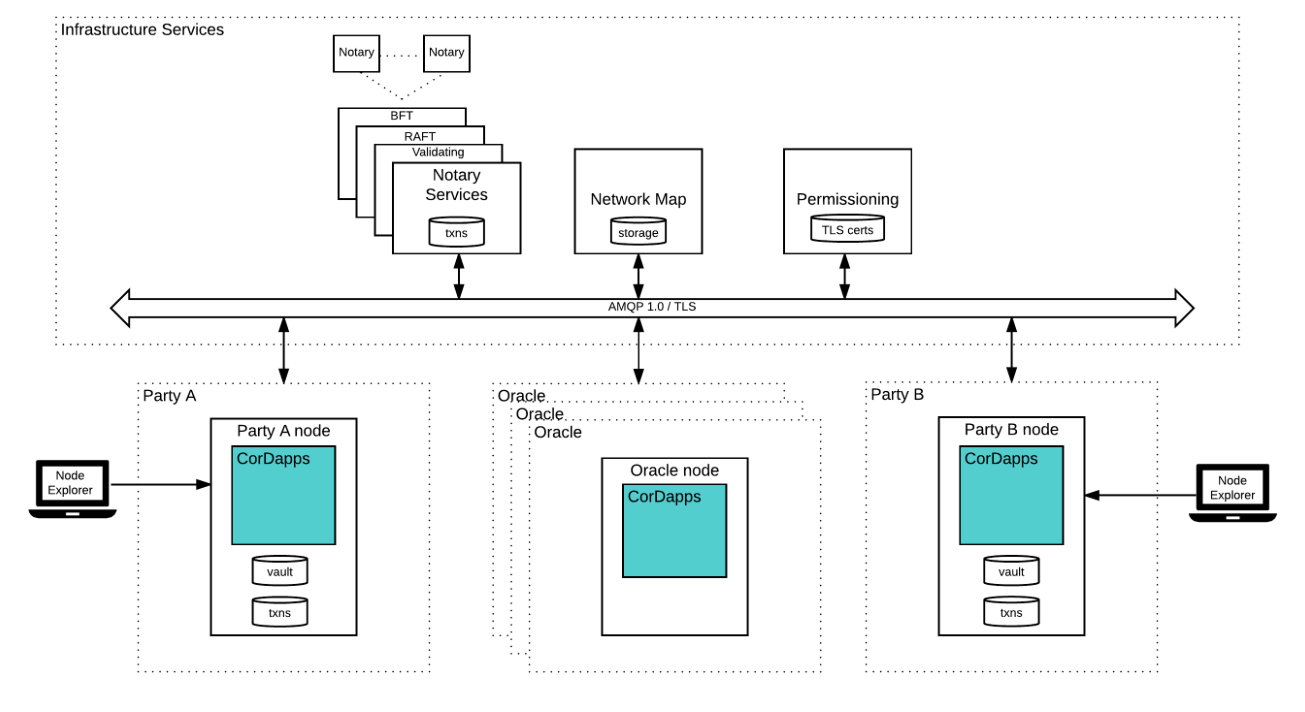
\includegraphics[width=\textwidth]{Figures/corda_architecture.png}
    \caption{Corda's architecture \cite{Hearn2016Corda:Ledger}}
    \label{fig:corda_architecture}
\end{figure}.
The Party A and Party B are two of the limited number of nodes possible who interact and transact between each other. Assigning a node to each user won't be scalable. This was contrary to the project idea for this thesis and consequently, the idea was dropped.


\section{Anchoring data to Blockchain}
Due to time and technical constraints, the whole idea of creating smart contract on a blockchain was dropped and instead the plan for utilising the already existing Bitcoin blockchain was made. This plan was fulfilled by the concept called anchoring of data on Bitcoin blockchain.
\\The use of the Bitcoin blockchain to timestamp and verify data in an immutable public ledger was pioneered by Manuel Aráoz with the creation of Proof of Existence\cite{Araoz2013ProofExistence}. This system, and others like it, notarise data in the blockchain by calculating a hash of the data and publishing it in a Bitcoin transaction. By comparing the hash published in the blockchain with the hash of the same data, it's possible to verify that the data existed at a specific time, providing a mechanism to validate a timestamp.
\\Anchoring in blockchain simply means adding your data to Bitcoin blockchain to provide irrefutable time-stamps and non-repudiation \cite{Lemieux2017Blockchain:}. There are multiple services that provide anchoring service for valuable data. For this project, Chainpoint was selected as they have a simple to use (and still free) REST API called Tierion to anchor data to Bitcoin blockchain. Their API provides the anchoring service using anchoring standard they created, Chainpoint.
\\Chainpoint links a hash of the specified data to a blockchain and returns a timestamp proof. A Chainpoint service receives hashes which are aggregated together using a Merkle tree. The root of this tree is anchored in the Bitcoin and Ethereum blockchains. Throughout this process a Chainpoint proof is created and continually upgraded. The final Chainpoint proof defines a path of operations that cryptographically links the specified data to one or more blockchains.\cite{ChainpointStandard}
\\A Chainpoint proof is a JSON-LD document which contains the information to cryptographically verify a piece of data is anchored to a blockchain. It proves the data existed at the time it was anchored. Chainpoint proofs can be verified without reliance on a trusted third party.
\footnote{JSON-LD is a lightweight Linked Data format described here \url{https://json-ld.org/}}
\\Once the data is sent to Tierion through their API, they generate a unique SHA 256 hash of the data. Multiple hashes are assembled into a block, which is simply a list of hashes. Periodically, these blocks are used to generate a Merkle Tree\cite{Merkle1980ProtocolsCryptosystems} , and the Merkle Root is published in the blockchain via a transaction. By collating multiple hashes into a Merkle Tree and publishing the Merkle Root, large volumes of data is anchored in the blockchain using a single transaction. \cite{Wayne2016Chainpoint:Receipts}

\subsection{Blockchain receipts}
Once the data is anchored, the insurance platform should also be able to provide the proof that the data has been hashed to the blockchain network and can be verified via third party too. In the real world, a receipt provides proof of a transaction. In this project's case, a blockchain receipt provides proof that some data existed at a specific time. It contains all the information needed to prove an individual hash was part of the Merkle Tree whose root was published in a transaction in the Blockchain. The data in the blockchain receipt is given in table \ref{table:receipt} and the use of fields to verify data is visually represented in figure \ref{fig:merkle}
\begin{table}[h!]
\centering
\begin{tabular}{||c c||} 
\hline
Name & Description  \\ [0.5ex] 
\hline\hline
@context & the JSON-LD context for the receipt \\ 
\hline
type & receipt type definition specifying hash method and version \\
\hline
targetHash & hash value being anchored to the blockchain \\
\hline
merkleRoot	& merkle tree root value that is anchored to the blockchain \\
\hline
proof	& merkle proof establishing a link from the targetHash to the merkleRoot \\
\hline
anchor-type	& anchor type definition specifying anchoring method \\
\hline
anchor-sourceId &	identifier, such as a transaction id, used to locate anchored data \\ [1ex]
 \hline
\end{tabular}
\caption{Different fields in blockchain receipt}
\label{table:receipt}
\end{table}

\begin{figure}[ht]
    \centering
    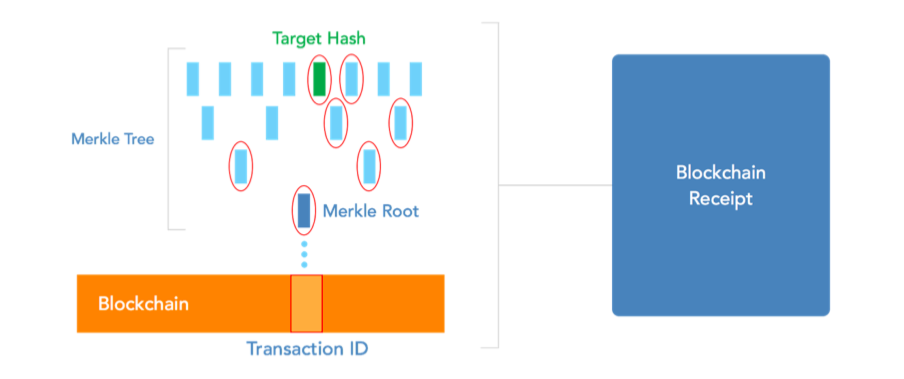
\includegraphics[width=\textwidth]{Figures/Merkle.png}
    \caption{Visual explanation of concept behind blockchain receipt\cite{Wayne2016Chainpoint:Receipts}}
    \label{fig:merkle}
\end{figure}

By tracing a path from the Merkle root to the target hash, a Merkle Proof can be generated that proves any one of the elements is in the Merkle tree, without having to know the entire tree.

\subsection{Integration with project}
The integration of data with Tierion was completed as explained in the following sequence:
\begin{itemize}
    \item Once the user selects and agrees to the shown insurance rates, a JSON string is created with user, flight and insurance data.
    \item The JSON string is sent to Tierion using REST API.
    \item A unique ID of the transaction is received as a response back from Tierion.
    \item Initially the status of the blockchain in unpublished and blockchain receipt is not received. However, within 10 minutes, the status is updated to published and the blockchain receipt is received. ID received earlier is used for updating the status of the transaction and blockchain receipt.
\end{itemize}